% !TeX spellcheck = de_DE
\section{NeuroEvolution of Augmenting Topologies}
\label{sec:neat}
Der in dieser Arbeit verwendete Algorithmus ist mit \ac{NEAT} bezeichnet und 2002 erstmals von \citeauthor{stanley2002evolving} vorgestellt worden. Zum Zeitpunkt der Veröffentlichung hat \ac{NEAT} für die meisten Optimierungsprobleme im Vergleich zu anderen Verfahren schneller Lösungen gefunden, obwohl es neben den Gewichten des \ac{KNN} auch die Struktur optimiert \cite{stanley2002evolving}. Dementsprechend gehört der Algorithmus zur Gruppe der \ac{TWEANN} Verfahren. Heute gilt \ac{NEAT} nach wie vor als einer der bekanntesten Vertreter der neuroevolutionären Algorithmen und dient als Basis für viele Erweiterungen wie zum Beispiel HyperNEAT \cite{stanley2009hyperneat}.
Für den großen Erfolg von \ac{NEAT} sind drei Eigenschaften besonders relevant \cite{stanley2002evolving}:
\begin{enumerate}
	\item Erfolgreiche Reproduktion trotz verschiedener Strukturen
	\item Schützen von neuen Innovationen durch verschiedene Spezies
	\item Wachsen einer minimalen Struktur
\end{enumerate}
In diesem Kapitel wird die grundsätzliche Funktionsweise von \ac{NEAT} erläutert, wie sie in der originalen Publikation vorgestellt ist. Wenn nicht anderweitig gekennzeichnet, beziehen sich alle Informationen aus diesem Kapitel auf Quelle \cite{stanley2002evolving}. Für eine bessere Lesbarkeit wird in diesem Kapitel auf weiteres Zitieren verzichtet.
\subsection{Kodierung}
\label{subsec:neat_encoding}
\begin{figure}[!h]
	\centering
	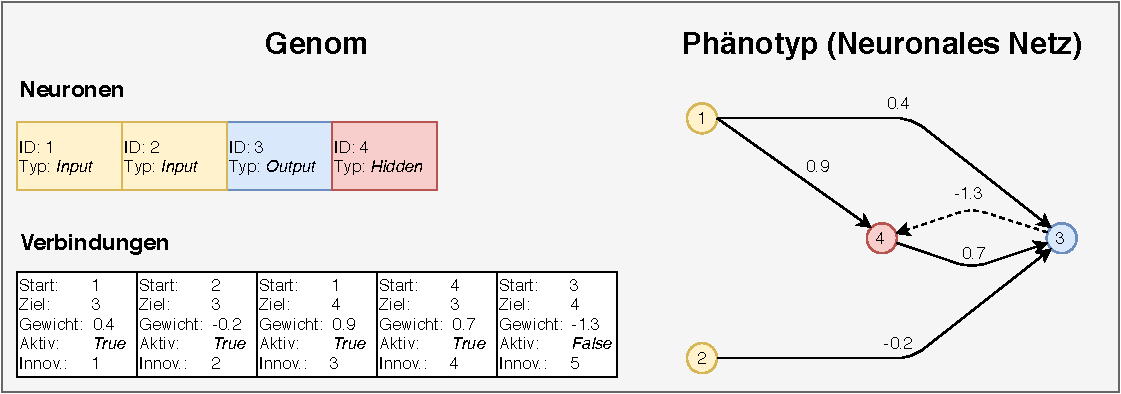
\includegraphics[width=1\textwidth]{./img/neat_genome_encoding.pdf} 
	\caption{Schematische Darstellung von einem Genom mit dazugehörigem Phänotyp}
	\label{fig:neat_encoding}
\end{figure}
\noindent
\ac{NEAT} verwendet ein direktes Kodierungsverfahren. Ein Genom enthält, wie in Abbildung \ref{fig:neat_encoding} beispielhaft dargestellt, je eine Liste für Neuronen und Verbindungen. Ein Neuron wird durch eine ID identifiziert und enthält einen Typ (\emph{Input}, \emph{Output} oder \emph{Hidden}). Eine Verbindung enthält das Start- und Zielneuron, das dazugehörige Gewicht, ein Aktivierungsbit sowie eine Innovationsnummer. Das Aktivierungsbit gibt an, ob die Verbindung im Phänotyp, in diesem Fall dem neuronalen Netz, enthalten ist. Auf die Funktionsweise und Bedeutung der Innnovationsnummer wird später genauer eingegangen.
\subsection{Mutation}
\label{subsec:neat_mutation}
Ein Genom kann auf verschiedene Arten mutieren, welche entweder die Struktur des \ac{KNN} oder die Gewichte der Verbindungen beeinflussen. Die Mutation der Gewichte ist ähnlich zu anderen neuroevolutionären Algorithmen. Für jedes Gewicht besteht eine Wahrscheinlichkeit zur Mutation. In diesem Fall wird das Gewicht entweder leicht abgeändert oder ein neuer zufälliger Wert gewählt.
\begin{figure}[!h]
	\centering
	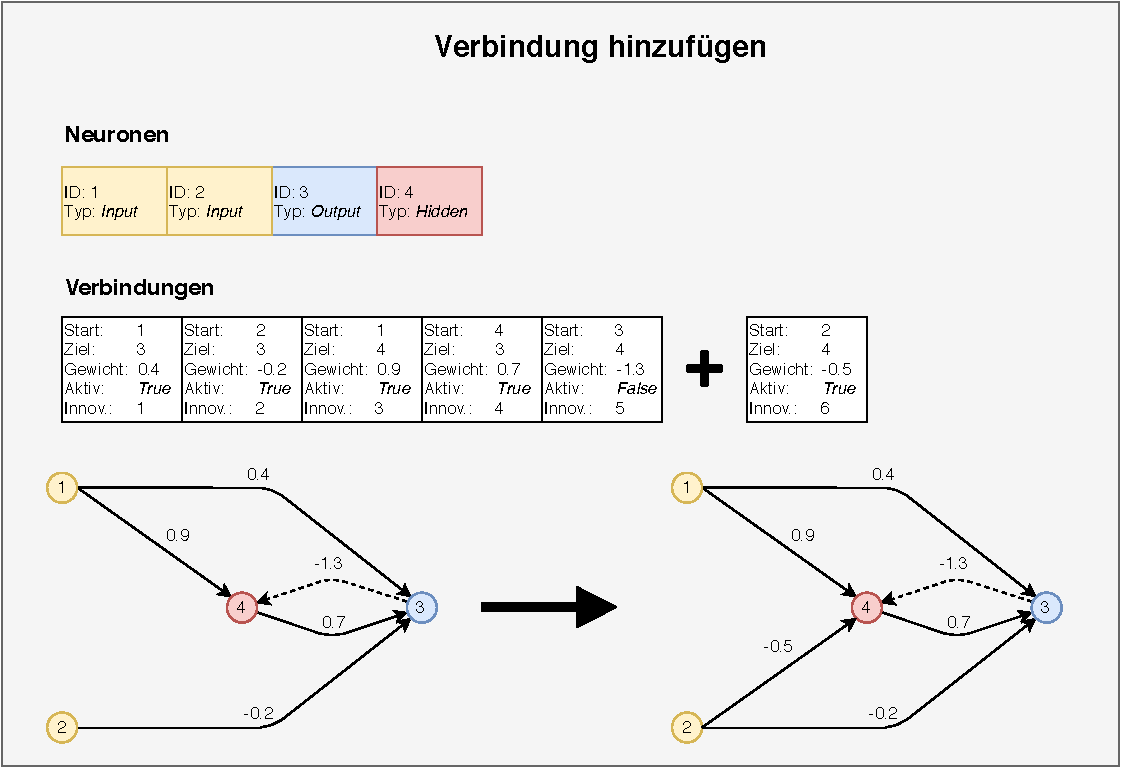
\includegraphics[width=1\textwidth]{./img/neat-AddConnectionMutation.pdf} 
	\caption{Schematische Darstellung einer strukturellen Mutation, bei der eine neue Verbindung zwischen den Neuronen $2$ und $4$ hinzugefügt wird}
	\label{fig:neat_add_connectin_mutation}
\end{figure}
\\ \noindent
Strukturelle Mutationen können in zwei verschiedenen Arten auftreten. Bei der ersten wird eine einzelne neue, vorher nicht vorhandene Verbindung dem Genom hinzugefügt. Das Gewicht für diese neue Verbindung wird zufällig gewählt und das Aktivierungsbit auf \emph{True} gesetzt. Ein Beispiel für die erste Art der strukturellen Mutation ist in Abbildung \ref{fig:neat_add_connectin_mutation} dargestellt. Die zweite Art der strukturellen Mutation sieht das Einfügen eines neuen Neurons in das \ac{KNN} vor. Hierzu wird zu Beginn eine aktive Verbindung $con_{ij} $ zufällig ausgewählt, welche von Neuron $i$ zu Neuron $j$ führt. Anschließend wird ein neues Neuron $x$ zwischen den Neuronen $i$ und $j$ platziert und zwei weitere Verbindungen werden hinzugefügt. Die erste Verbindung $con_{ix}$ führt vom alten Startneuron $i$ zum neu hinzugefügtem und erhält das Gewicht $1$. Die zweite Verbindung $con_{xj}$ beginnt beim neuen Neuron und endet im alten Zielneuron $j$ und erhält dasselbe Gewicht wie die Verbindung $con_{ij}$. Zuletzt wird die ausgewählte Verbindung $con_{ij}$ deaktiviert, indem das Aktivierungsbit auf $False$ gesetzt wird. Diese Art der Mutation reduziert den initialen Effekt des neuen Neurons, sodass es ohne eine starke Optimierung direkt vom \ac{KNN} verwendet werden kann.
\begin{figure}[!h]
	\centering
	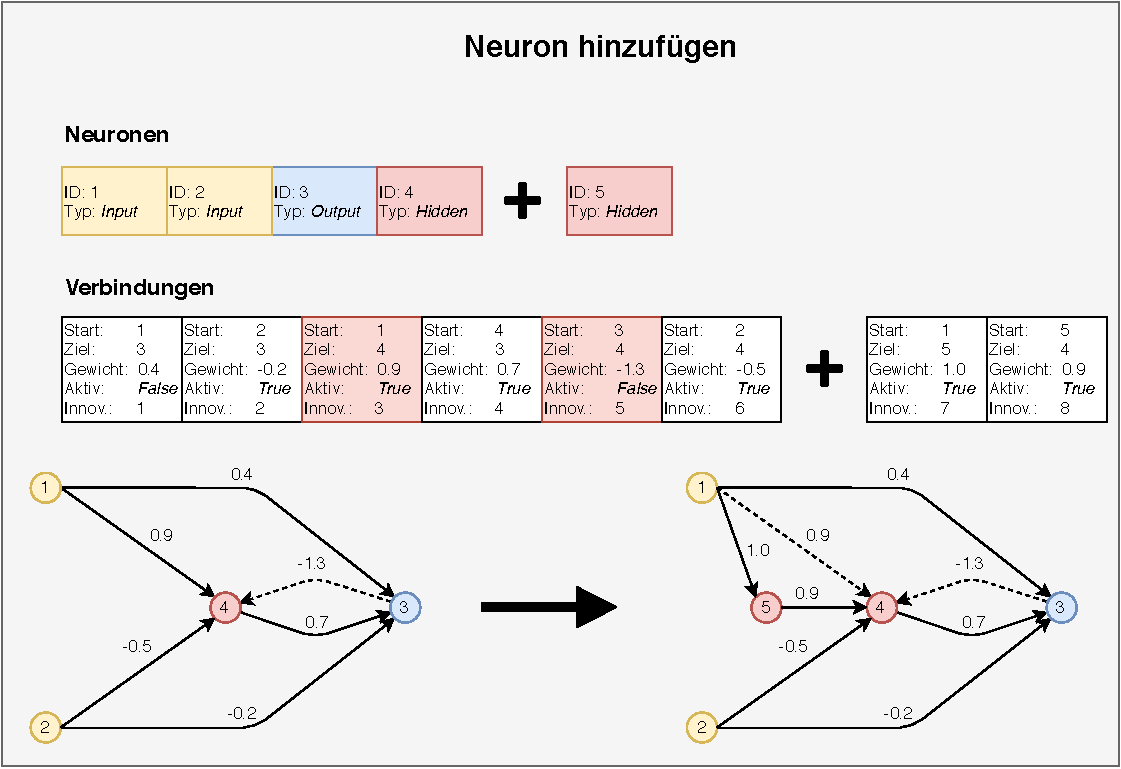
\includegraphics[width=1\textwidth]{./img/neat-AddNodeMutation.pdf} 
	\caption{Schematische Darstellung einer strukturellen Mutation, bei der ein neues Neuron zwischen den Neuronen $1$ und $4$ hinzugefügt wird}
	\label{fig:neat_add_node_mutation}
\end{figure}
\subsection{Reproduktion}
\label{subsec:neat_reproduction}
Das Ergebnis der in Kapitel \ref{subsec:neat_mutation} vorgestellten Mutationen ist eine Population mit verschiedenen Genomen mit potenziell unterschiedlichen Gewichten und Strukturen. Dies ist die schwierigste Form des in Kapitel \ref{subsubsec:recombination} vorgestellten \emph{Competing Conventions} Problems und macht das Erstellen von Nachkommen besonders schwierig. \ac{NEAT} löst dieses Problem, indem es den historischen Ursprung von jeder strukturellen Mutation überwacht. Haben zwei Verbindungen denselben Ursprung, haben sie in der Vergangenheit dieselbe Struktur repräsentiert, auch wenn sie inzwischen unterschiedliche Gewichte haben. Zu diesem Zweck besitzt jede Verbindungen eine entsprechende Innovationsnummer. Mit jeder Entstehung einer neuen Verbindung wird ein globaler Zähler erhöht, woraufhin dieser Wert der Verbindung als Innovationsnummer zugewiesen wird. Die Abbildungen \ref{fig:neat_add_connectin_mutation} und \ref{fig:neat_add_node_mutation} zeigen diese Zuweisung beispielhaft. Werden die Verbindungen eines Genoms in der Reproduktionsphase für die Nachkommen ausgewählt, wird auch die Innovationsnummer übertragen. Somit ist auch bei den nachfolgenden Generationen ersichtlich, was der historische Ursprung einer Verbindung ist. Tritt durch Zufall dieselbe Mutation in einer Generation mehrfach auf, erhalten die neuen Verbindungen dieselben Innovationsnummern. Hierfür müssen alle aufgetretenen Mutationen einer Generation zwischengespeichert werden. 
\\\\
Die Innovationsnummern können nicht nur ressourcensparend implementiert werden, sie erleichtern auch das Erzeugen von Nachkommen in der Reproduktionsphase dahingehend, dass beim Kreuzen von zwei Elternteilen keine aufwendige Strukturanalyse erforderlich ist. Die sogenannten \emph{maching genes} sind Verbindungen, deren Innovationsnummern in beiden Elterngenomen vorkommen. Beim Erstellen der Nachkommen wird für jede Verbindung in den \emph{matching genes} zufällig entschieden, aus welchem Elternteil diese übernommen wird. Die sogenannten \emph{disjoint genes} und \emph{excess genes} sind Verbindungen, die nur in einem Elternteil vorkommen. Zu den \emph{disjoint genes} gehören diejenigen Verbindungen, deren Innovationsnummer kleiner als die größte Innovationsnummer des zweiten Elterngenoms ist. Die \emph{excess genes} sind Verbindungen, deren Innovationsnummer größer als die höchste Innovationsnummer im anderen Elternteil ist. Beim Erzeugen von Nachkommen werden nur die \emph{excess genes} und \emph{disjoint genes} von dem Elternteil übernommen, welches den höheren Fitnesswert erzielt hat. Haben beide Elternteile denselben Wert, werden die Verbindungen beider übernommen. 
Bei dieser Implementierung wird angenommen, dass der Schwellwert der Neuronen, wie in Kapitel \ref{subsec:optimization_strategies} erläutert, durch eine Verbindung zu einem \emph{Bias}-Neuron ausgedrückt wird. Dadurch enthalten die Neuronen keine spezifischen Informationen und werden bei der Reproduktion immer vom Elternteil mit dem höheren Fitnesswert übernommen.
\subsection{Spezies}
\label{subsec:neat_species}
Die vorgestellten Arten der Mutation und die erfolgreiche Reproduktion ermöglichen es \ac{NEAT}, eine Population mit vielen verschiedenen Strukturen zu entwickeln. Dennoch reichen diese Faktoren nicht aus, da in der Praxis neue strukturelle Innovationen nur eine geringe Chance haben, langfristig integriert zu werden und es wahrscheinlicher ist, dass sie nach wenigen Generation aussterben. Die Gründe hierfür sind, dass kleinere \ac{KNN} schneller optimiert werden können als große und dass das Hinzufügen von neuen Neuronen und Verbindungen den Fitnesswert meist initial senkt, auch wenn die neuen Strukturen für das erfolgreiche Lösen des Optimierungsproblems notwendig sind. So folgt letztendlich, dass die kleinen Genome anfänglich bessere Fitnesswerte erzielen, sodass die größeren Genome nicht für die Reproduktion ausgewählt werden, wodurch die strukturellen Innovationen wieder verloren gehen.
\\\\
Das Problem wird von \ac{NEAT} durch die Einführung verschiedener Spezies gelöst. Das Ziel ist, Genome, die sich strukturell ähnlich sind, in einer Spezies zu gruppieren. Bei der Auswahl der Elterngenome für die Nachkommen muss ein Genom nicht mehr mit der ganzen Population konkurrieren, sondern nur noch mit den anderen Genomen der eigenen Spezies. Somit sind neue Innovationen erst einmal in ihrer Spezies vor dem Aussterben geschützt und können mit der Zeit optimiert werden. Für die Implementierung eines solchen Verfahrens wird eine Funktion benötigt, die messen kann, wie ähnlich oder unterschiedlich zwei Genome sind. Auch hier kann wie bei der Rekombination auf eine aufwendige Strukturanalyse verzichtet werden, da die bereits bekannten Innovationsnummern für die Umsetzung einer entsprechenden Implementierung genutzt werden können. Je mehr \emph{excess genes} und \emph{disjoint genes} zwei Genome besitzen, desto weniger evolutionäre Geschichte teilen sie und sind somit unterschiedlicher. Nicht zuletzt ist auch der Gewichtsunterschied ein entscheidender Faktor. Die von \ac{NEAT} verwendete Formel, um die Kompatibilität $\delta$ zwischen zwei Genomen zu berechnen, ist im Folgenden abgebildet:
$$\delta=\frac{c_1E}{N}+\frac{c_2D}{N}+c_3 \cdot \overline{W}$$
Die Variablen $E$ und $D$ ergeben sich aus der Anzahl an \emph{excess genes} und \emph{disjoint genes}. $\overline{W}$ beschreibt die durchschnittliche Gewichtsdifferenz der \emph{matching genes}. Die Faktoren $c_1$, $c_2$ und $c_3$ ermöglichen es, die Wichtigkeit der einzelnen Komponenten je nach Optimierungsproblem zu justieren. $N$ steht für die Anzahl der Verbindungen im größeren Genom und normalisiert die Anzahl der \emph{excess genes} und \emph{disjoint genes}, sodass in großen Genomen der Effekt auf den Kompatibilitätswert $\delta$ bei einer neuen Verbindung gering, in kleinen hingegen sehr groß ist. Je nach Konfiguration kann für kleine Genome $N=1$ gelten.
\\\\
Die Zuordnung von neu erstellten Genomen zu einer Spezies erfolgt im Anschluss an die Reproduktions- und Mutationsphase. Hierfür wird eine geordnete Liste mit allen verfügbaren Spezies benötigt. Jede Spezies wird durch ein Genom repräsentiert, welches in der vorherigen Generation ein Mitglied von dieser war. Bei der Zuordnung von einem Genom wird über die Liste der Spezies iteriert und zu jedem Repräsentanten der Kompatibilitätswert $\delta$ gebildet. Ist $\delta \leq \delta_t$, wobei $\delta_t$ ein konfigurierbarer Schwellwert ist, wird das Genom der Spezies zugeordnet und die Suche abgebrochen. Ist das Genom zu keiner Spezies kompatibel, wird eine neue erstellt und das Genom als deren Repräsentant gesetzt.
\\\\
Zum Erhalten verschiedener Strukturen muss verhindert werden, dass eine Spezies zu groß wird und die restlichen verdrängt, auch wenn viele der Mitglieder gute Fitnesswerte erzielen. Zusätzlich müssen insbesondere neue Spezies geschützt werden. Diese haben initial wenige Mitglieder und damit eine geringere Chance, als Elterngenome ausgewählt zu werden. Zum Lösen dieses Problems verwendet \ac{NEAT} sogenanntes \emph{explicit fitness sharing}, welches \citeauthor{goldberg1987genetic} 1987 in ihrer Arbeit vorstellen \cite{goldberg1987genetic}. Jeder Spezies wird bei der Reproduktion eine Anzahl an Nachkommen zugewiesen, welche proportional zur Fitness $f_{s}$ der Spezies ist. Diese ergibt sich aus der Summe aller angepassten Fitnesswerte $f'$ der Mitglieder. Der angepasste Fitnesswert $f'$ eines Genoms wird mithilfe des Quotienten aus der Fitness $f$ und der Anzahl an Mitgliedern der Spezies gebildet. Ziel dieser Maßnahme ist, dass große Spezies im Vergleich zu kleinen benachteiligt werden. Hierdurch werden kleineren erfolgreichen Spezies entsprechend viele Nachkommen zugeordnet.
\\\\
Ist der Fitnesswert $f_s$ jeder Spezies berechnet und die Nachkommen proportional zugeteilt, beginnt die Reproduktion. Die Elterngenome werden hierfür zufällig aus den besten $50\%$ der Mitglieder der entsprechenden Spezies ausgewählt. Sind alle Nachkommen erstellt, wird die gesamte Population gelöscht und durch die Nachkommen ersetzt. Diese werden nach dem bereits vorgestellten Verfahren wieder den Spezies zugeordnet.

\subsection{Starten mit einer minimalen Struktur}
\label{subsec:neat_minimal_structure}
Das Ziel von \ac{NEAT} sowie vieler anderer Optimierungsalgorithmen ist, eine Lösung in kürzester Zeit zu finden. Einen wichtigen Faktor stellt hierbei die Größe des \ac{KNN} dar. Ein zu großes \ac{KNN} hat viele modifizierbare Verbindungsgewichte und Schwellwerte, welche nicht für die erfolgreiche Lösung benötigt werden, aber dennoch zu optimieren sind. Dadurch erhöht sich die Laufzeit des Algorithmus. Ein zu kleines \ac{KNN} kann hingegen, wie in Kapitel \ref{subsec:xor_implementation} veranschaulicht, unter Umständen nicht in der Lage sein, eine Lösung zu finden. Dementsprechend ist die richtige Größe des \ac{KNN} entscheidend für die schnelle Optimierung. Für Algorithmen, welche nur die Gewichte eines \ac{KNN} optimieren, muss diese Struktur manuell festgelegt werden. Meistens basiert dies auf Expertenwissen oder Erfahrung \cite{stanley2017oreilly}. Im Gegensatz hierzu stehen die \ac{TWEANN} Algorithmen, welche selbstständig eine gute Struktur bilden sollen. Diese starten oft mit einer initialen Population mit vielen verschiedenen zufällig erstellten Topologien, um anfänglich genetische Diversität zu bieten. Wie in Kapitel \ref{subsubsec:mutation} erläutert, ist dies oft ineffizient, da viele Strukturen nicht gebraucht werden und Zeit aufzuwenden ist, sie zu entfernen.
\\\\
\ac{NEAT} hingegen startet mit einer Population, bei der alle Genome dieselbe minimale Struktur besitzen. Die entstehenden \ac{KNN} haben ausschließlich \emph{Input}- und \emph{Output}-, nicht jedoch \emph{Hidden}-Neuronen. Jedes \emph{Input}-Neuron besitzt eine Verbindung zu jedem \emph{Output}-Neuron mit einem zufällig gewählten Gewicht. Neue Strukturen werden durch die vorgestellten Arten der Mutation hinzugefügt, von denen nur diejenigen langfristig integriert werden, welche den Fitnesswert erhöhen. Somit ist die Existenz jeder Struktur in einem Genom gerechtfertigt. Insgesamt ergibt sich daraus für \ac{NEAT} ein Vorteil bezüglich der Evaluationszeit anderen \ac{TWEANN} Algorithmen gegenüber, da die Anzahl der zu optimierenden Parameter und somit die Dimensionen des Suchraums minimiert sind.